\subsection{Servo (CG)}
\label{sec:servo}
%TODO CG Write chapter

\subsubsection{Requirements}
First of all, all specified requirements except one optional one were fulfilled. In detail the three braking and one steering servos are controlled and the Pololu Maestro Mini Servo Controller Board was connected to them and checked for functionality. The optional requirement to control the main engine was not fulfilled for several reasons. First off all time was running out at the end of the project due to several faced difficulties described in chapter~\ref{sec:challenges}. Furthermore the main engine ca not be controlled by the Pololu Maestro Mini Servo Controller board, because of its power consumption. Instead another more complex controller needs to be used, which requires a serial connection. However Genode as an operating system only supports one serial connection. That is why an additional device would have been needed to be integrated into the setup to control it.

\subsubsection{Hardware Description}
As already described in section~\ref{sec:setup} the used hardware consists of three braking servos, one steering servo and a pololu maestro mini servo controller board, which is displayed in figure~\ref{fig:pololu}.\\

All four servo engines are controlled with a 50Hz pulse width modulation(PWM) signal as is standard for servo engines. The duty cycle of each PWM-signal is between 1 and 2 milliseconds. Because of the nature of the servo controller board, values for the duty cycle of a PWM signal need to be between 4000 and 8000, which corresponds to four times the value in microseconds.\\

\begin{figure}[h!tb]
	\centering
    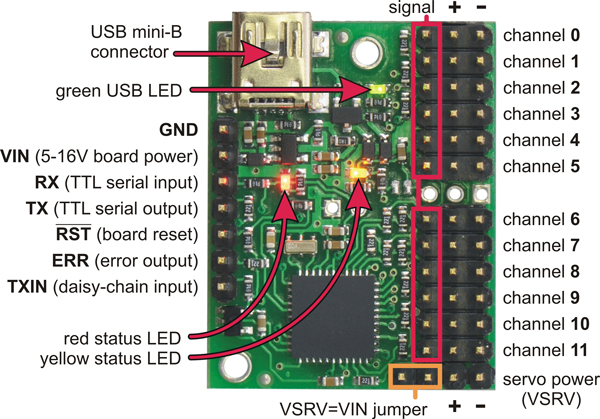
\includegraphics[width=0.7\linewidth]{images/pololu}
    \caption{Pololu Maestro Mini}
    \label{fig:pololu}
\end{figure}

The installed controller board features twelve PWM channels which need to be run on the same frequency but support different duty cycles, so that up to 12 servos could be controlled. For communication with a computer serial communication via USB or UART/TTL on a byte basis can be used. The baudrate for the UART connection is normally autodetected and can be configure. Messages are always sent as eight bits without parity bit and one stop bit(8N1). It also has the capability to execute small script programs. The braking servos are connected to channel 0,1 and 2 and the steering servo is connected to channel 6.\\

Initially the steering servo was not working and therefore was replaced by the chair. Additionally we configured it after its replacement. Also the braking servos were tried to be configured to engage at the same time. However the made improvement was only minor.

\subsubsection{Software Description}
For first testing a shell script and an interactive program with a graphical user interface, both working on all common operating systems, are provided by the supplier and were used. Also some small c example code is provided and was used as a starting point during development. The shell script and the example code is for reference located in the old/pololu folder described in chapter~\ref{sec:scs}.\\

Because of delays in the installation of Genode on the Raspberry Pi that is communicating with the servo controller board, a first program was developed for controlling the servos on Linux, especially Raspbian. The serial port used for communication is exposed as a file in Linux. Therefore commands can be send by writing into the correct file. The program can be found in the old/linux folder as described in chapter~\ref{sec:scs}.\\

All functions provided by the servo class/component have a similar structure. First the input values are checked for valid range, second a command is built and sent and lastly its return value checked for errors. If the servo controller board is supposed to answer, the response is read in, checked for errors and returned. Each command is represented as a char array, where the 7 least significant bits represent one serial message. The first message is always the actual command type, the next one is the channel that is affected and lastly a value is sent often split up into two messages in little-endian format.\\

Only little changes were needed to port the code to Genode. Additionally the program was made a complete component, which can be called via remote procedure calls(RPC), which lead to several difficulties. The exposed functions are documented in chapter~\ref{sec:api}. How the code is used on the Raspberry PI is described in more detail in the following chapter~\ref{sec:rpi}.